\documentclass{article}

\usepackage{graphicx}
\usepackage{tikz}
\usepackage{tikzsymbols}
\usetikzlibrary{calc,patterns,shapes.geometric}
\pagestyle{empty}
\usepackage[margin=0pt]{geometry}
\geometry{papersize={14in,12in}}

\def\centerarc[#1](#2)(#3:#4:#5){\draw[#1] ($(#2)+({#5*cos(#3)},{#5*sin(#3)})$) arc (#3:#4:#5);}

\begin{document}
	\begin{figure}
		\centering
		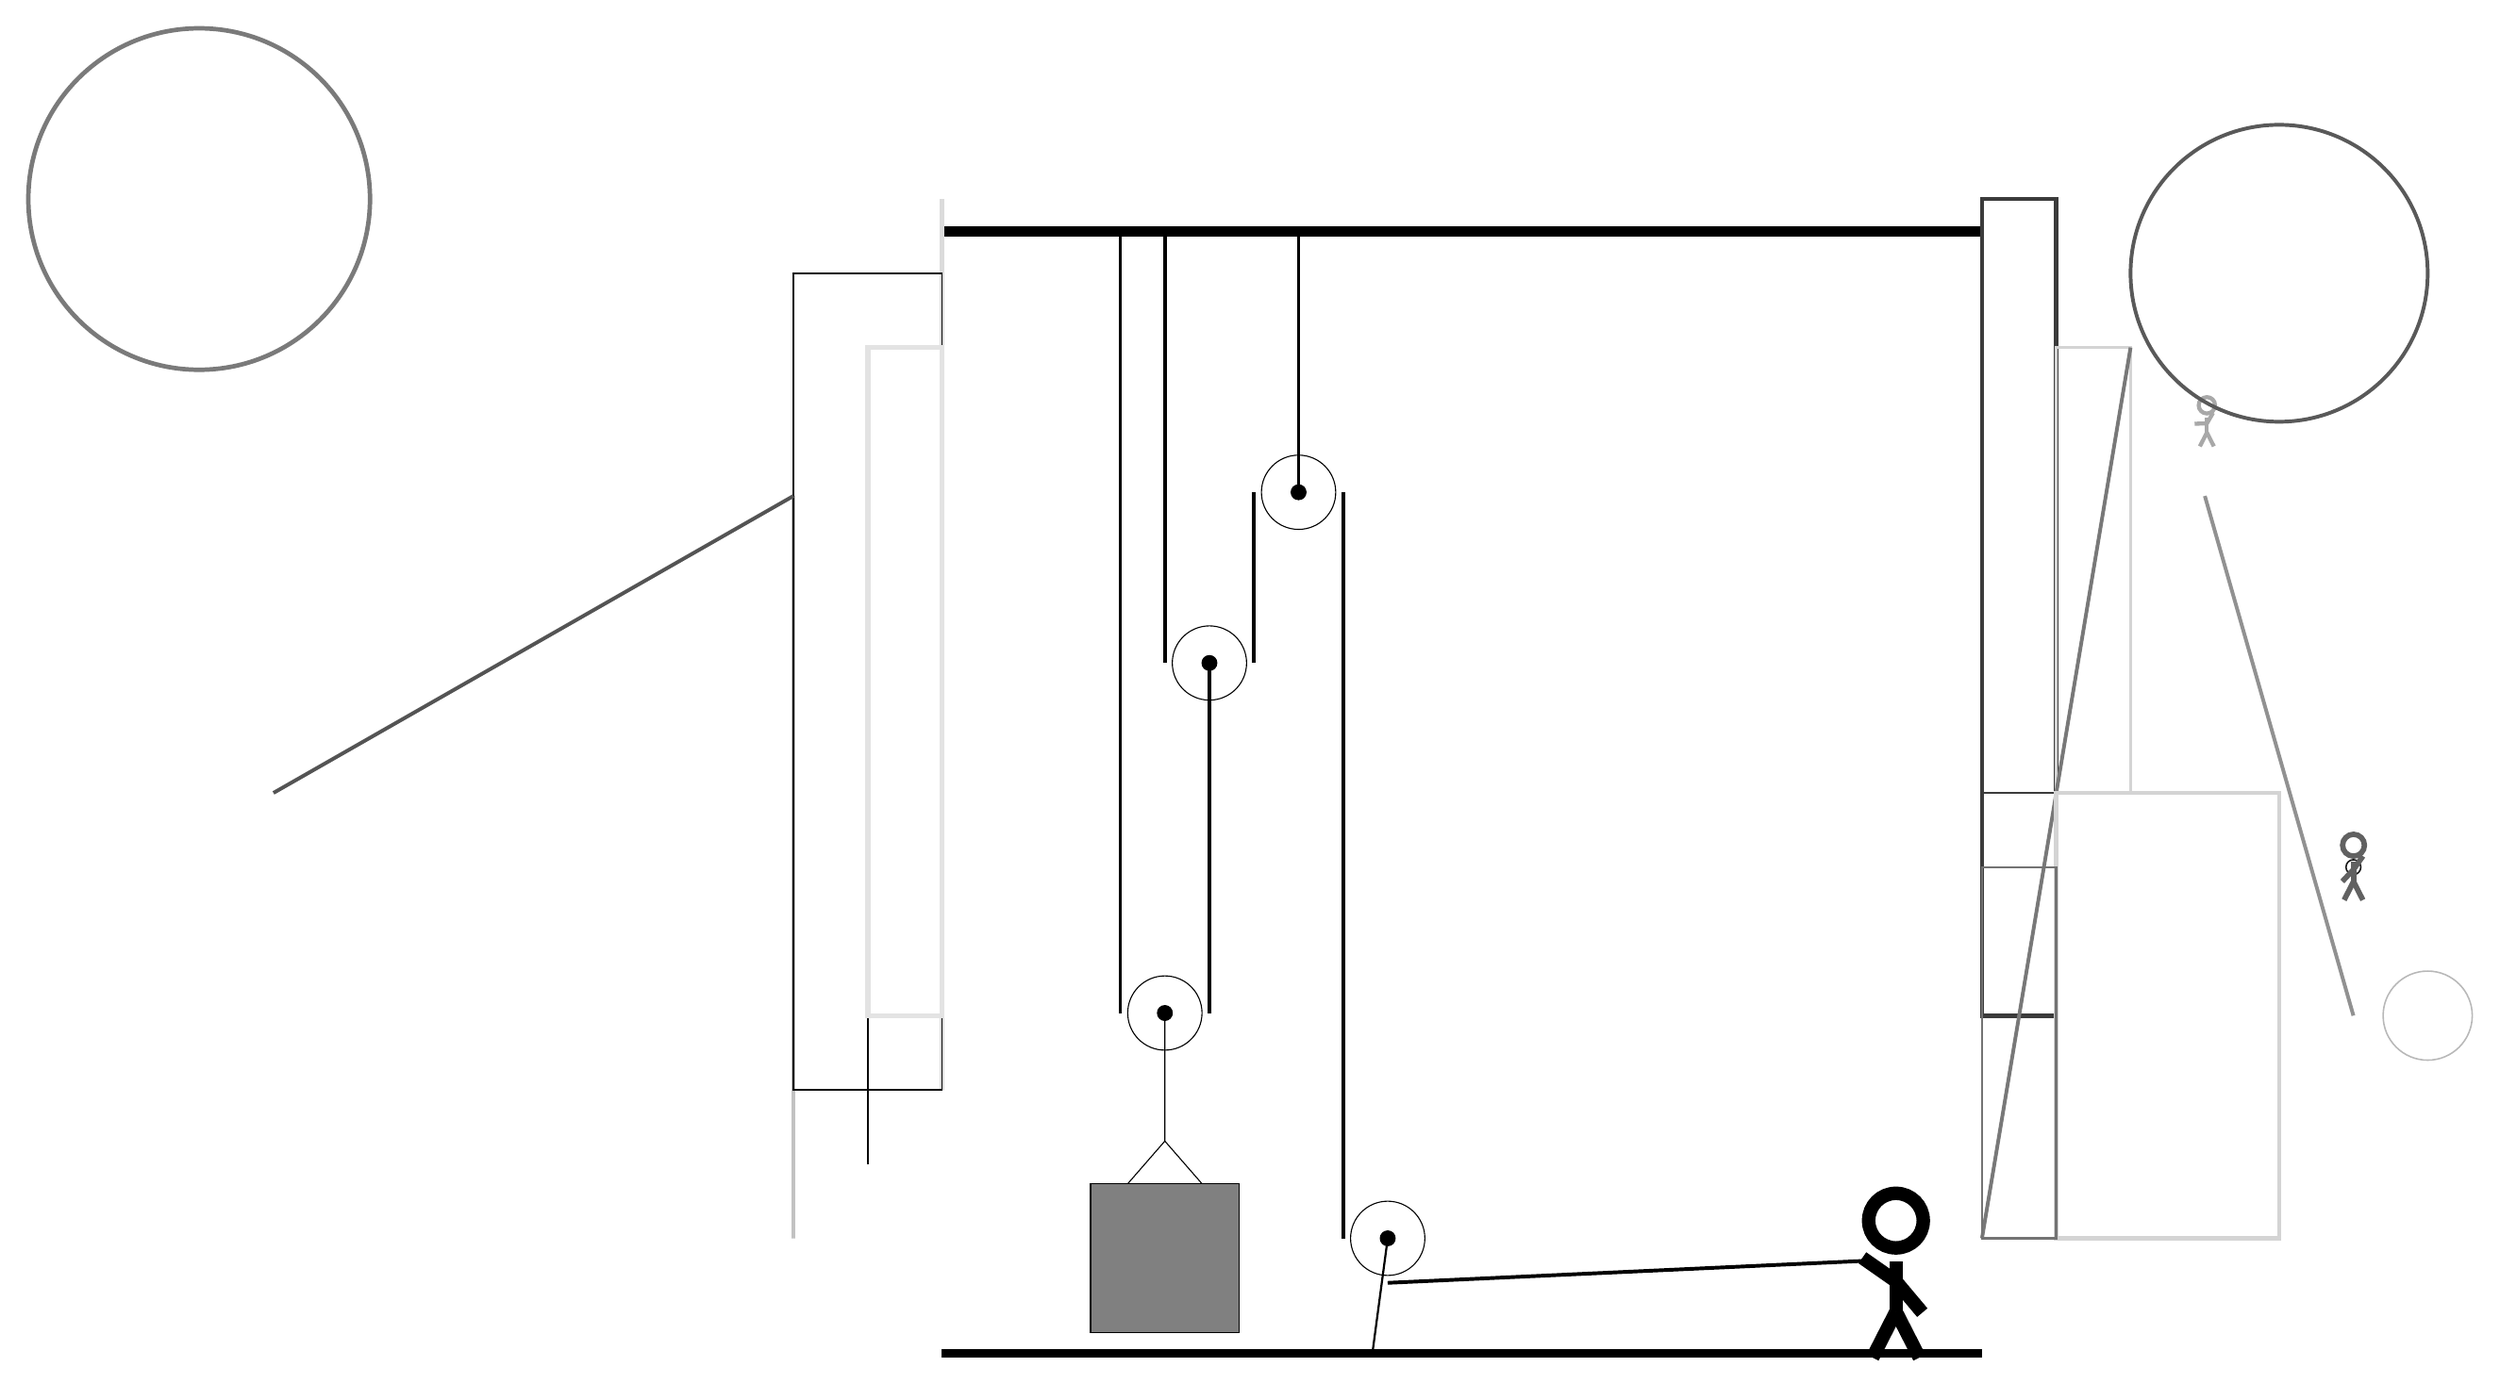
\begin{tikzpicture}
			%%%%% START %%%%%
			
			\draw[fill=black] (-2, 11.5) rectangle (12, 11.625);
			
			\draw (1, 1.035) circle (0.5);
			\draw[fill=black] (1, 1.035) circle (0.1);
			
			\draw (1.6, 5.75) circle (0.5);
			\draw[fill=black] (1.6, 5.75) circle (0.1);
			
			\draw (2.8, 8.05) circle (0.5);
			\draw[fill=black] (2.8, 8.05) circle (0.1);
			\draw[thick] (2.8, 8.05) -- (2.8, 11.5);
			
			\draw (4.0, -2) circle (0.5);
			\draw[fill=black] (4.0, -2) circle (0.1);
			\draw[thick] (4.0, -2) -- (3.8, -3.5);
			
			\draw [line width=0.2mm, color=black!91](17, 3) circle (0.1);
			
			\node[line width=0.5mm, color=black!34] at (15, 9) {\Strichmaxerl[3][1][60]};
			\draw [line width=0.2mm, color=black!28](18, 1) circle (0.6);
			\node[line width=0.4mm, color=black!62] at (17, 3) {\Strichmaxerl[4][47][55]};
			\draw[line width=0.6mm, color=black!14] (-2, 0) rectangle (-2, 12);
			\draw[line width=0.2mm, color=black!96] (12, 11) rectangle (12, -1);
			\draw [line width=0.5mm, color=black!65](16, 11) circle (2.0);
			\draw[line width=0.6mm, color=black!77] (12, 12) rectangle (13, 1);
			\draw[line width=0.3mm, color=black!17] (13, 10) rectangle (14, 4);
			
			\draw[line width=0.4mm, color=black!24] (-4, 8) rectangle (-4, -2);
			
			\draw[line width=0.2mm, color=black!77] (12, 4) rectangle (14, 4);
			
			\draw[line width=0.2mm, color=black!97] (-3, -1) rectangle (-3, 1);
			\draw[line width=0.2mm, color=black!96] (-2, 11) rectangle (-4, 0);
			\draw[line width=0.7mm, color=black!11] (-2, 1) rectangle (-3, 10);
			\draw[line width=0.5mm, color=black!53](14, 10) -- (12, -2);
			\draw[line width=0.6mm, color=black!17] (13, 4) rectangle (16, -2);
			
			\draw[line width=0.5mm, color=black!67](-4, 8) -- (-11, 4);
			\draw [line width=0.6mm, color=black!52](-12, 12) circle (2.3);
			\draw[line width=0.3mm, color=black!55] (13, -2) rectangle (12, 3);
			\draw[line width=0.5mm, color=black!43](17, 1) -- (15, 8);
			
			\draw (1, 1.035) -- (1, -0.69) -- (0.5, -1.265) -- (1.5, -1.265) -- (1, -0.69);
			\draw[fill=black!50] (0, -1.265) rectangle (2, -3.265);
			\draw[line width=0.5mm] (0.4, 11.5) -- (0.4, 1.035);
			\centerarc[line width=0.5mm](1, 1.035)(180:360:0.6);
			\draw[line width=0.5mm](1.6, 1.035) -- (1.6, 5.75);
			\draw[line width=0.5mm] (1.0, 11.5) -- (1.0, 5.75);
			\centerarc[line width=0.5mm](1.6, 5.75)(180:360:0.6);
			\draw[line width=0.5mm](2.2, 5.75) -- (2.2, 8.05);
			\centerarc[line width=0.5mm](2.8, 8.05)(0:180:0.6);
			\draw[line width=0.5mm] (3.4, 8.05) -- (3.4, -2);
			\centerarc[line width=0.5mm](4.0, -2)(0:90:-0.6);
			\draw[line width=0.5mm](4.0, -2.6) -- (10.5, -2.3);
			
			\node at (10.8, -2.5) {\Strichmaxerl[10][-35][-50]};
			
			\draw[fill=black] (-2, -3.5) rectangle (12, -3.6);
			
			%%%%% END %%%%%
		\end{tikzpicture}
	\end{figure}	
\end{document}